% Introduction et présentation du problème

\begin{document}

\begin{frame}
  \titlepage
\end{frame}

\begin{frame}{Plan de la présentation}
  \tableofcontents
\end{frame}

\section{Introduction}

\begin{frame}{Contexte et problématique}
  \begin{itemize}
    \item<1-> \textbf{Contexte:} Gestion des feux tricolores à un carrefour à 4 voies
    \item<2-> \textbf{Problématique:} Comment minimiser le temps d'attente des véhicules?
    \item<3-> \textbf{Approche:} 
    \begin{itemize}
      \item Modélisation formelle avec Event-B pour garantir la sécurité
      \item Implémentation d'un algorithme adaptatif d'optimisation
    \end{itemize}
  \end{itemize}
  
  \vspace{0.5cm}
  \onslide<4->{
  \begin{center}
    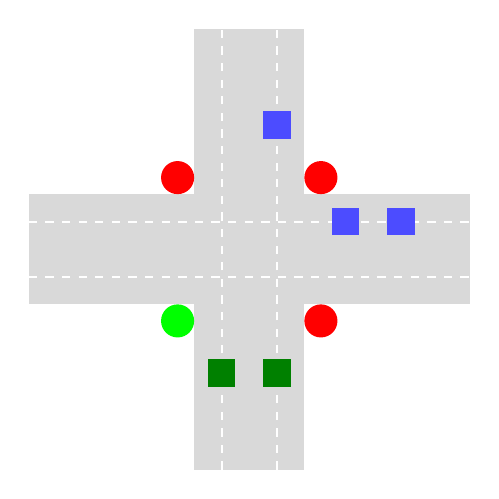
\begin{tikzpicture}[scale=0.7]
      % Routes
      \fill[gray!30] (-4,0) rectangle (4,1);
      \fill[gray!30] (-4,-1) rectangle (4,0);
      \fill[gray!30] (0,-4) rectangle (1,4);
      \fill[gray!30] (-1,-4) rectangle (0,4);
      
      % Lignes de route
      \draw[white, dashed, thick] (-4,0.5) -- (4,0.5);
      \draw[white, dashed, thick] (-4,-0.5) -- (4,-0.5);
      \draw[white, dashed, thick] (0.5,-4) -- (0.5,4);
      \draw[white, dashed, thick] (-0.5,-4) -- (-0.5,4);
      
      % Feux tricolores
      \fill[red] (1.3,1.3) circle (0.3);
      \fill[green] (-1.3,-1.3) circle (0.3);
      \fill[red] (1.3,-1.3) circle (0.3);
      \fill[red] (-1.3,1.3) circle (0.3);
      
      % Véhicules
      \fill[blue!70] (2.5,0.25) rectangle (3,0.75);
      \fill[blue!70] (1.5,0.25) rectangle (2,0.75);
      \fill[blue!70] (0.25,2) rectangle (0.75,2.5);
      \fill[green!50!black] (0.25,-2) rectangle (0.75,-2.5);
      \fill[green!50!black] (-0.25,-2) rectangle (-0.75,-2.5);
    \end{tikzpicture}
  \end{center}}
\end{frame}

\begin{frame}{Objectifs du projet}
  \begin{enumerate}
    \item<1-> \textbf{Modéliser formellement} le système de feux tricolores avec Event-B
    \begin{itemize}
      \item Garantir qu'il n'y aura jamais de feux verts simultanés pour des directions conflictuelles
      \item Assurer la sécurité des piétons
    \end{itemize}
    
    \item<2-> \textbf{Concevoir un algorithme adaptatif} pour minimiser les temps d'attente
    \begin{itemize}
      \item Ajuster dynamiquement les durées des phases en fonction des files d'attente
      \item Respecter les contraintes de sécurité définies dans le modèle formel
    \end{itemize}
    
    \item<3-> \textbf{Intégrer et implémenter} la solution dans une simulation JavaScript
    \begin{itemize}
      \item Visualiser le comportement du système optimisé
      \item Mesurer les gains de performance par rapport à des durées fixes
    \end{itemize}
  \end{enumerate}
\end{frame}

\section{Modélisation formelle avec Event-B}

\begin{frame}{Event-B : présentation}
  \begin{itemize}
    \item<1-> \textbf{Event-B} : méthode formelle basée sur la théorie des ensembles et la logique du premier ordre
    \item<2-> \textbf{Avantages pour notre système de feux tricolores:}
    \begin{itemize}
      \item Modélisation précise des états et transitions
      \item Vérification formelle des propriétés de sécurité
      \item Raffinement progressif du système abstrait vers l'implémentation
    \end{itemize}
  \end{itemize}
  
  \onslide<3->{
  \begin{center}
    \begin{tikzpicture}[node distance=1.5cm, auto]
      % Définir les styles
      \tikzstyle{block} = [rectangle, draw, fill=blue!20, text width=8em, text centered, rounded corners, minimum height=3em]
      \tikzstyle{line} = [draw, -latex']
      
      % Nœuds principaux
      \node [block] (context) {Contexte Event-B};
      \node [block, right=of context] (machine) {Machine Event-B};
      \node [block, below=of context] (const) {Constantes\\Axiomes};
      \node [block, below=of machine] (vars) {Variables\\Invariants\\Événements};
      
      % Connections
      \path [line] (context) -- (machine);
      \path [line] (context) -- (const);
      \path [line] (machine) -- (vars);
    \end{tikzpicture}
  \end{center}}
\end{frame}

\begin{frame}[fragile]{Contexte Event-B: TrafficLightContext}
  \begin{lstlisting}[style=EventB]
CONTEXT TrafficLightContext

CONSTANTS
    MIN_PHASE_DURATION,    // Durée minimale
    MAX_PHASE_DURATION,    // Durée maximale
    yellow_duration,       // Durée du feu jaune
    MAX_QUEUE_LENGTH,      // Longueur maximale de file
    OPTIMIZATION_INTERVAL  // Intervalle d'optimisation

AXIOMS
    MIN_PHASE_DURATION = 10 &
    MAX_PHASE_DURATION = 60 &
    yellow_duration = 3 &
    MAX_QUEUE_LENGTH = 50 &
    OPTIMIZATION_INTERVAL = 20
END
  \end{lstlisting}
  
  \begin{itemize}
    \item Les constantes définissent les paramètres immuables du système
    \item Les axiomes fixent les valeurs concrètes des constantes
  \end{itemize}
\end{frame}

\begin{frame}[fragile]{Machine Event-B: TrafficLightControl (1/2)}
  \begin{lstlisting}[style=EventB]
MACHINE TrafficLightControl

SEES TrafficLightContext

SETS
    DIRECTIONS = {NORTH, SOUTH, EAST, WEST};
    COLORS = {RED, YELLOW, GREEN};
    PEDESTRIAN_SIGNALS = {WALK, DONT_WALK};
    PHASES = {PHASE_NS, PHASE_EW, TRANSITION_NS_TO_EW, TRANSITION_EW_TO_NS}

VARIABLES
    traffic_lights,      // État des feux
    pedestrian_signals,  // État des signaux piétons
    current_phase,       // Phase actuelle
    timer,               // Temps écoulé
    queue_length,        // Longueur des files
    waiting_time         // Temps d'attente cumulé
  \end{lstlisting}
\end{frame}

\begin{frame}[fragile]{Machine Event-B: TrafficLightControl (2/2)}
  \begin{lstlisting}[style=EventB]
INVARIANTS
    // Typage des variables
    traffic_lights ∈ DIRECTIONS → COLORS &
    pedestrian_signals ∈ DIRECTIONS → PEDESTRIAN_SIGNALS &
    current_phase ∈ PHASES &
    timer ∈ ℕ &
    queue_length ∈ DIRECTIONS → ℕ &
    
    // Propriété de sécurité fondamentale:
    // Les feux opposés ne peuvent pas être verts simultanément
    ∀d1, d2 · (d1 ∈ DIRECTIONS & d2 ∈ DIRECTIONS & 
              ((d1 = NORTH & d2 = EAST) or 
               (d1 = NORTH & d2 = WEST) or
               (d1 = SOUTH & d2 = EAST) or 
               (d1 = SOUTH & d2 = WEST))) ⇒
              ¬(traffic_lights(d1) = GREEN & 
                traffic_lights(d2) = GREEN)
  \end{lstlisting}
  
  \begin{itemize}
    \item Les invariants garantissent le typage correct des variables
    \item L'invariant de sécurité empêche les collisions potentielles
  \end{itemize}
\end{frame}
